\section{Partial Redundancy Elimination}
\begin{flushright}
\textit{Notes by Akshin Singh}
\end{flushright}

A particularly good place to optimize is in loops. Since loops can run for a million iterations, moving any computation from 
inside the loop to outside while maintaing correctness is a desirable optimization. Such kind of optimization is called loop invariant
code motion. 

\begin{figure}[h]
\centering
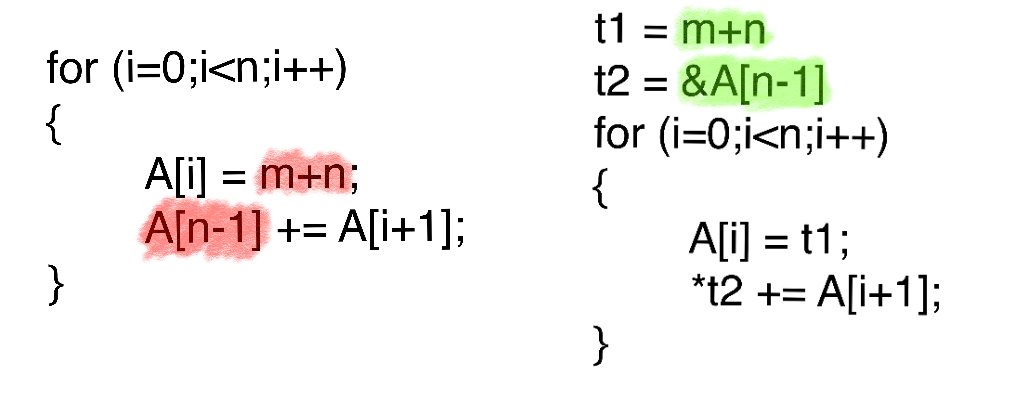
\includegraphics[scale = 0.5]{images/mod_105_fig1.png}
\caption{Loop invariant Code Motion Example}
\label {fig:mod_105_01}
\end{figure}

Let us explain with the help of an example. See the original code present in Figure \ref{fig:mod_105_01}. Since i is the loop variable,
that gets incremented every iteration, both \textbf{A[i]} and \textbf{A[i+1]} are dependent on the loop's progress. Hence these variables
are not invariant. However, the expression \textbf{m+n} and \textbf{A[n-1]} are both loop invariant. This is because both n and m hold their
values across iterations. We can therefore transform the code as shown.

Notice that since we have removed an addition as well as an address calculation (which is a multiply and add instruction), we have reduced
the number of instructions in the loop by two. Now if the loop runs a million times, we have saved a lot of work (typically on the order of 
two to three hunderd cycles). 

What happens if the loop does not run even once? Our transformed code will then have two extra instructions and we have inadvertently slowed
ourseleves by optimizing. This is the tradeoff that an optimizing compiler decides to make or not. 

\subsection{Partial Redundancy Elimination}

Let us take a deeper look into why we wanted to transform code in \ref{fig:mod_105_01}. Let us try to follow the control of the program.
We enter the program and then enter the loop. Inside the loop we calculate \textbf{m+n} and \textbf{A[n-1]} in the first iteration. 
Then, before the values of m and n are changed we subsequently calculated \textbf{m+n} and \textbf{A[n-1]} again in the next iteration. 

Keeping this in mind, let us define the problem of Partial Redundancy. If an expression is redundant (we will 
define redundancy in a while) on any path leading to it, it is said to be partially redundant. This is not the case in Common subexpression
elimination, where we can remove only those expressions which are completely redundant, i.e., redundant on all paths. 

\begin{figure}[h]
\centering
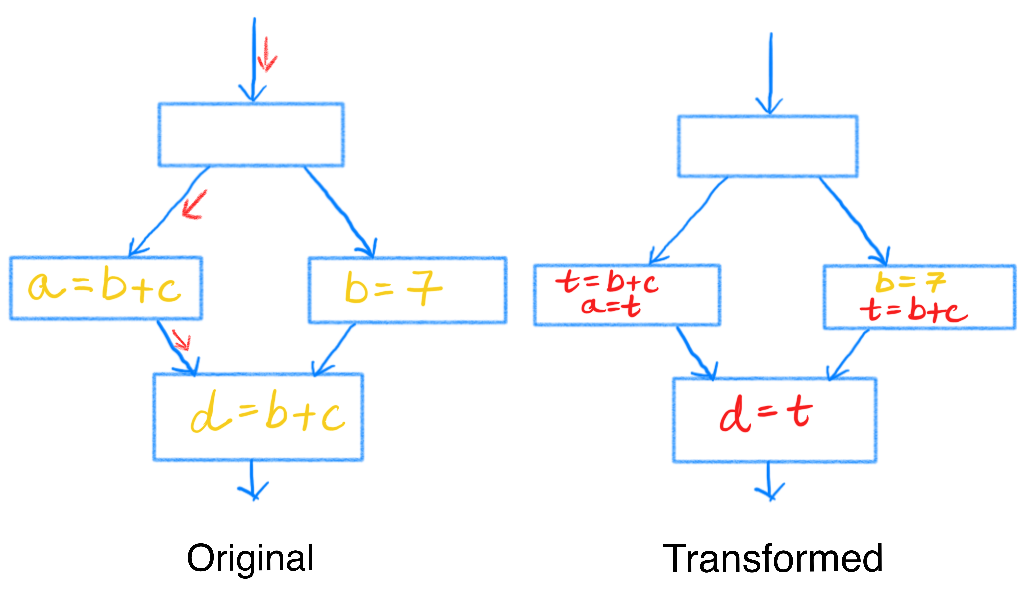
\includegraphics[scale = 0.5]{images/mod_105_fig2.png}
\caption{Partial Redundancy Elimination Example}
\label {fig:mod_105_02}
\end{figure}

A clearer example can be seen in Figure \ref{fig:mod_105_02}. Here \textbf{b+c} is redundant on the path from \textbf{a=b+c} and not on the 
other path. The transformed code has no redundancy. Partial Redundancy Elimination (or PRE for short) is the problem of placing computations (like \textbf{a=b+c}) such that no path recomputes
the same expression.

\begin {itemize}
\item Since PRE is a general optimization that does not need to work on only loops, PRE subsumes Loop invariant code motion. This is because
any computation that is loop invariant is redundant on the path that goes from the loop body back to the loop body.  

\begin{figure}[h]
\centering
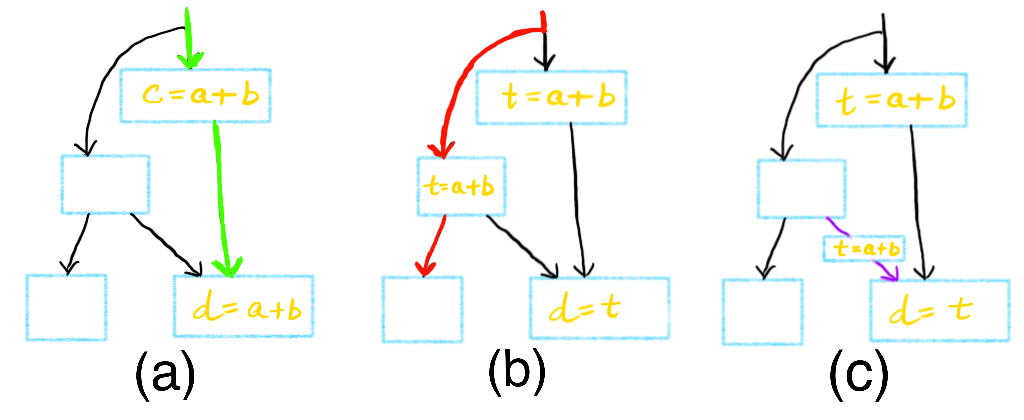
\includegraphics[scale = 0.3]{images/mod_105_fig3.png}
\caption{Redundancy Example}
\label {fig:mod_105_03}
\end{figure}

\item PRE may require addition of basic blocks. To understand this we need to define redundancy. Let us first take an example. Figure 
\ref{fig:mod_105_03}(a) has a redundancy on the green path. If the computation is moved as shown in \ref{fig:mod_105_03}(b), we have
a problem on the red path. The problem is that \textbf{a+b} is not needed anywhere on that path, and yet it is being computed. Naturally we
only want those computations to be present on a path that will be used eventually on that path. This leads us to define redundancy as 
any computation on a path that is either happening more than once if needed or at least once if not needed. To solve the problem, we need 
to add a basic block as shown in \ref{fig:mod_105_03}(c). Only then can we remove all partial redundancies.

Formally, the problem arised from the fact that we are hoisting computation across a \textbf{critical edge}. A critical edge is an edge
in the CFG where the source block has multiple successors and the desitination block has multiple predecessors. Hoisting across a critical
edge requires a new basic block since we may add redundancy on other paths. The pruple edge in \ref{fig:mod_105_03}(c) is the critical edge.

\item Even after adding basic blocks, there can be cases where we cannot elimate PRE until we decide to duplicate the code. See the 
Figure \ref{fig:mod_105_04}(a).

\begin{figure}[h]
\centering
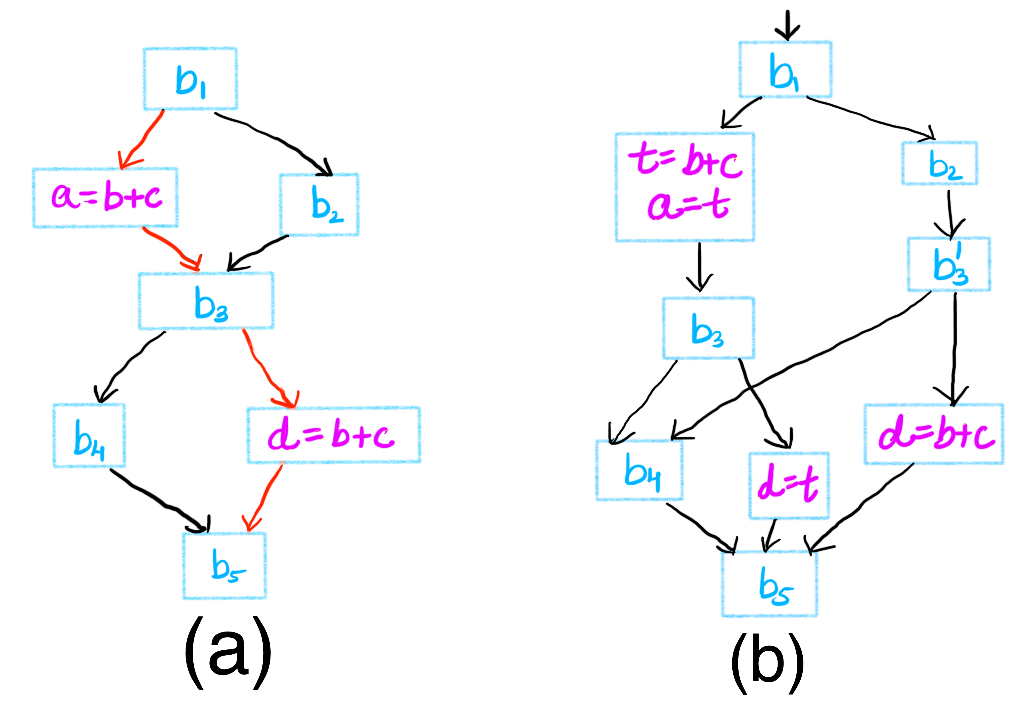
\includegraphics[scale = 0.3]{images/mod_105_fig4.png}
\caption{PRE Duplication Example}
\label {fig:mod_105_04}
\end{figure}

Here the expression \textbf{b+c} is redundant on the red path as shown. Here we need to duplicate the code as shown in 
Figure \ref{fig:mod_105_04}(b). Code duplication has caching effects. A larger code-size means a jump can be a jump to 
a far instruction which may incur a cache-miss which is not desirable, especially in today's out-of-order 6-8 wide issue processors. 
The penalty for i-cache miss can be very high. 
\end{itemize}